
%% bare_conf.tex
%% V1.4b
%% 2015/08/26
%% by Michael Shell
%% See:
%% http://www.michaelshell.org/
%% for current contact information.
%%
%% This is a skeleton file demonstrating the use of IEEEtran.cls
%% (requires IEEEtran.cls version 1.8b or later) with an IEEE
%% conference paper.
%%
%% Support sites:
%% http://www.michaelshell.org/tex/ieeetran/
%% http://www.ctan.org/pkg/ieeetran
%% and
%% http://www.ieee.org/

%%*************************************************************************
%% Legal Notice:
%% This code is offered as-is without any warranty either expressed or
%% implied; without even the implied warranty of MERCHANTABILITY or
%% FITNESS FOR A PARTICULAR PURPOSE! 
%% User assumes all risk.
%% In no event shall the IEEE or any contributor to this code be liable for
%% any damages or losses, including, but not limited to, incidental,
%% consequential, or any other damages, resulting from the use or misuse
%% of any information contained here.
%%
%% All comments are the opinions of their respective authors and are not
%% necessarily endorsed by the IEEE.
%%
%% This work is distributed under the LaTeX Project Public License (LPPL)
%% ( http://www.latex-project.org/ ) version 1.3, and may be freely used,
%% distributed and modified. A copy of the LPPL, version 1.3, is included
%% in the base LaTeX documentation of all distributions of LaTeX released
%% 2003/12/01 or later.
%% Retain all contribution notices and credits.
%% ** Modified files should be clearly indicated as such, including  **
%% ** renaming them and changing author support contact information. **
%%*************************************************************************


% *** Authors should verify (and, if needed, correct) their LaTeX system  ***
% *** with the testflow diagnostic prior to trusting their LaTeX platform ***
% *** with production work. The IEEE's font choices and paper sizes can   ***
% *** trigger bugs that do not appear when using other class files.       ***                          ***
% The testflow support page is at:
% http://www.michaelshell.org/tex/testflow/



\documentclass[conference]{IEEEtran}
% Some Computer Society conferences also require the compsoc mode option,
% but others use the standard conference format.
%
% If IEEEtran.cls has not been installed into the LaTeX system files,
% manually specify the path to it like:
% \documentclass[conference]{../sty/IEEEtran}





% Some very useful LaTeX packages include:
% (uncomment the ones you want to load)


% *** MISC UTILITY PACKAGES ***
%
%\usepackage{ifpdf}
% Heiko Oberdiek's ifpdf.sty is very useful if you need conditional
% compilation based on whether the output is pdf or dvi.
% usage:
% \ifpdf
%   % pdf code
% \else
%   % dvi code
% \fi
% The latest version of ifpdf.sty can be obtained from:
% http://www.ctan.org/pkg/ifpdf
% Also, note that IEEEtran.cls V1.7 and later provides a builtin
% \ifCLASSINFOpdf conditional that works the same way.
% When switching from latex to pdflatex and vice-versa, the compiler may
% have to be run twice to clear warning/error messages.






% *** CITATION PACKAGES ***
%
%\usepackage{cite}
% cite.sty was written by Donald Arseneau
% V1.6 and later of IEEEtran pre-defines the format of the cite.sty package
% \cite{} output to follow that of the IEEE. Loading the cite package will
% result in citation numbers being automatically sorted and properly
% "compressed/ranged". e.g., [1], [9], [2], [7], [5], [6] without using
% cite.sty will become [1], [2], [5]--[7], [9] using cite.sty. cite.sty's
% \cite will automatically add leading space, if needed. Use cite.sty's
% noadjust option (cite.sty V3.8 and later) if you want to turn this off
% such as if a citation ever needs to be enclosed in parenthesis.
% cite.sty is already installed on most LaTeX systems. Be sure and use
% version 5.0 (2009-03-20) and later if using hyperref.sty.
% The latest version can be obtained at:
% http://www.ctan.org/pkg/cite
% The documentation is contained in the cite.sty file itself.






% *** GRAPHICS RELATED PACKAGES ***
%
\ifCLASSINFOpdf
  % \usepackage[pdftex]{graphicx}
  % declare the path(s) where your graphic files are
  % \graphicspath{{../pdf/}{../jpeg/}}
  % and their extensions so you won't have to specify these with
  % every instance of \includegraphics
  % \DeclareGraphicsExtensions{.pdf,.jpeg,.png}
\else
  % or other class option (dvipsone, dvipdf, if not using dvips). graphicx
  % will default to the driver specified in the system graphics.cfg if no
  % driver is specified.
  % \usepackage[dvips]{graphicx}
  % declare the path(s) where your graphic files are
  % \graphicspath{{../eps/}}
  % and their extensions so you won't have to specify these with
  % every instance of \includegraphics
  % \DeclareGraphicsExtensions{.eps}
\fi
% graphicx was written by David Carlisle and Sebastian Rahtz. It is
% required if you want graphics, photos, etc. graphicx.sty is already
% installed on most LaTeX systems. The latest version and documentation
% can be obtained at: 
% http://www.ctan.org/pkg/graphicx
% Another good source of documentation is "Using Imported Graphics in
% LaTeX2e" by Keith Reckdahl which can be found at:
% http://www.ctan.org/pkg/epslatex
%
% latex, and pdflatex in dvi mode, support graphics in encapsulated
% postscript (.eps) format. pdflatex in pdf mode supports graphics
% in .pdf, .jpeg, .png and .mps (metapost) formats. Users should ensure
% that all non-photo figures use a vector format (.eps, .pdf, .mps) and
% not a bitmapped formats (.jpeg, .png). The IEEE frowns on bitmapped formats
% which can result in "jaggedy"/blurry rendering of lines and letters as
% well as large increases in file sizes.
%
% You can find documentation about the pdfTeX application at:
% http://www.tug.org/applications/pdftex





% *** MATH PACKAGES ***
%
%\usepackage{amsmath}
% A popular package from the American Mathematical Society that provides
% many useful and powerful commands for dealing with mathematics.
%
% Note that the amsmath package sets \interdisplaylinepenalty to 10000
% thus preventing page breaks from occurring within multiline equations. Use:
%\interdisplaylinepenalty=2500
% after loading amsmath to restore such page breaks as IEEEtran.cls normally
% does. amsmath.sty is already installed on most LaTeX systems. The latest
% version and documentation can be obtained at:
% http://www.ctan.org/pkg/amsmath





% *** SPECIALIZED LIST PACKAGES ***
%
%\usepackage{algorithmic}
% algorithmic.sty was written by Peter Williams and Rogerio Brito.
% This package provides an algorithmic environment fo describing algorithms.
% You can use the algorithmic environment in-text or within a figure
% environment to provide for a floating algorithm. Do NOT use the algorithm
% floating environment provided by algorithm.sty (by the same authors) or
% algorithm2e.sty (by Christophe Fiorio) as the IEEE does not use dedicated
% algorithm float types and packages that provide these will not provide
% correct IEEE style captions. The latest version and documentation of
% algorithmic.sty can be obtained at:
% http://www.ctan.org/pkg/algorithms
% Also of interest may be the (relatively newer and more customizable)
% algorithmicx.sty package by Szasz Janos:
% http://www.ctan.org/pkg/algorithmicx




% *** ALIGNMENT PACKAGES ***
%
%\usepackage{array}
% Frank Mittelbach's and David Carlisle's array.sty patches and improves
% the standard LaTeX2e array and tabular environments to provide better
% appearance and additional user controls. As the default LaTeX2e table
% generation code is lacking to the point of almost being broken with
% respect to the quality of the end results, all users are strongly
% advised to use an enhanced (at the very least that provided by array.sty)
% set of table tools. array.sty is already installed on most systems. The
% latest version and documentation can be obtained at:
% http://www.ctan.org/pkg/array


% IEEEtran contains the IEEEeqnarray family of commands that can be used to
% generate multiline equations as well as matrices, tables, etc., of high
% quality.




% *** SUBFIGURE PACKAGES ***
%\ifCLASSOPTIONcompsoc
%  \usepackage[caption=false,font=normalsize,labelfont=sf,textfont=sf]{subfig}
%\else
%  \usepackage[caption=false,font=footnotesize]{subfig}
%\fi
% subfig.sty, written by Steven Douglas Cochran, is the modern replacement
% for subfigure.sty, the latter of which is no longer maintained and is
% incompatible with some LaTeX packages including fixltx2e. However,
% subfig.sty requires and automatically loads Axel Sommerfeldt's caption.sty
% which will override IEEEtran.cls' handling of captions and this will result
% in non-IEEE style figure/table captions. To prevent this problem, be sure
% and invoke subfig.sty's "caption=false" package option (available since
% subfig.sty version 1.3, 2005/06/28) as this is will preserve IEEEtran.cls
% handling of captions.
% Note that the Computer Society format requires a larger sans serif font
% than the serif footnote size font used in traditional IEEE formatting
% and thus the need to invoke different subfig.sty package options depending
% on whether compsoc mode has been enabled.
%
% The latest version and documentation of subfig.sty can be obtained at:
% http://www.ctan.org/pkg/subfig




% *** FLOAT PACKAGES ***
%
%\usepackage{fixltx2e}
% fixltx2e, the successor to the earlier fix2col.sty, was written by
% Frank Mittelbach and David Carlisle. This package corrects a few problems
% in the LaTeX2e kernel, the most notable of which is that in current
% LaTeX2e releases, the ordering of single and double column floats is not
% guaranteed to be preserved. Thus, an unpatched LaTeX2e can allow a
% single column figure to be placed prior to an earlier double column
% figure.
% Be aware that LaTeX2e kernels dated 2015 and later have fixltx2e.sty's
% corrections already built into the system in which case a warning will
% be issued if an attempt is made to load fixltx2e.sty as it is no longer
% needed.
% The latest version and documentation can be found at:
% http://www.ctan.org/pkg/fixltx2e


%\usepackage{stfloats}
% stfloats.sty was written by Sigitas Tolusis. This package gives LaTeX2e
% the ability to do double column floats at the bottom of the page as well
% as the top. (e.g., "\begin{figure*}[!b]" is not normally possible in
% LaTeX2e). It also provides a command:
%\fnbelowfloat
% to enable the placement of footnotes below bottom floats (the standard
% LaTeX2e kernel puts them above bottom floats). This is an invasive package
% which rewrites many portions of the LaTeX2e float routines. It may not work
% with other packages that modify the LaTeX2e float routines. The latest
% version and documentation can be obtained at:
% http://www.ctan.org/pkg/stfloats
% Do not use the stfloats baselinefloat ability as the IEEE does not allow
% \baselineskip to stretch. Authors submitting work to the IEEE should note
% that the IEEE rarely uses double column equations and that authors should try
% to avoid such use. Do not be tempted to use the cuted.sty or midfloat.sty
% packages (also by Sigitas Tolusis) as the IEEE does not format its papers in
% such ways.
% Do not attempt to use stfloats with fixltx2e as they are incompatible.
% Instead, use Morten Hogholm'a dblfloatfix which combines the features
% of both fixltx2e and stfloats:
%
% \usepackage{dblfloatfix}
% The latest version can be found at:
% http://www.ctan.org/pkg/dblfloatfix




% *** PDF, URL AND HYPERLINK PACKAGES ***
%
%\usepackage{url}
% url.sty was written by Donald Arseneau. It provides better support for
% handling and breaking URLs. url.sty is already installed on most LaTeX
% systems. The latest version and documentation can be obtained at:
% http://www.ctan.org/pkg/url
% Basically, \url{my_url_here}.




% *** Do not adjust lengths that control margins, column widths, etc. ***
% *** Do not use packages that alter fonts (such as pslatex).         ***
% There should be no need to do such things with IEEEtran.cls V1.6 and later.
% (Unless specifically asked to do so by the journal or conference you plan
% to submit to, of course. )
\usepackage{graphicx}
\usepackage{float}
\usepackage{algorithm}
\usepackage{algpseudocode}
\usepackage{amsmath}
\usepackage{booktabs}
%\usepackage[options ]{algorithm2e}
% correct bad hyphenation here
\hyphenation{op-tical net-works semi-conduc-tor}


\begin{document}
%
% paper title
% Titles are generally capitalized except for words such as a, an, and, as,
% at, but, by, for, in, nor, of, on, or, the, to and up, which are usually
% not capitalized unless they are the first or last word of the title.
% Linebreaks \\ can be used within to get better formatting as desired.
% Do not put math or special symbols in the title.
\title{Community Detection by modeling entity-annotated
text: A Non-Negative Matrix Factorization Approach.}


% author names and affiliations
% use a multiple column layout for up to three different
% affiliations
\author{\IEEEauthorblockN{Pranav Nerurkar}
\IEEEauthorblockA{Research Scholar,\\Dept. of Computer Engineering,\\
Veermata Jijabai Technological Institute,\\
Matunga (W), Mumbai - 400019.\\
Email: pranavn91@gmail.com}
\and
\IEEEauthorblockN{Sunil Bhirud}
\IEEEauthorblockA{Professor,\\Dept. of Computer Engineering,\\
Veermata Jijabai Technological Institute,\\
Matunga (W), Mumbai - 400019.\\
Email: sgbhirud@vjti.org.in}}

% conference papers do not typically use \thanks and this command
% is locked out in conference mode. If really needed, such as for
% the acknowledgment of grants, issue a \IEEEoverridecommandlockouts
% after \documentclass

% for over three affiliations, or if they all won't fit within the width
% of the page, use this alternative format:
% 
%\author{\IEEEauthorblockN{Michael Shell\IEEEauthorrefmark{1},
%Homer Simpson\IEEEauthorrefmark{2},
%James Kirk\IEEEauthorrefmark{3}, 
%Montgomery Scott\IEEEauthorrefmark{3} and
%Eldon Tyrell\IEEEauthorrefmark{4}}
%\IEEEauthorblockA{\IEEEauthorrefmark{1}School of Electrical and Computer Engineering\\
%Georgia Institute of Technology,
%Atlanta, Georgia 30332--0250\\ Email: see http://www.michaelshell.org/contact.html}
%\IEEEauthorblockA{\IEEEauthorrefmark{2}Twentieth Century Fox, Springfield, USA\\
%Email: homer@thesimpsons.com}
%\IEEEauthorblockA{\IEEEauthorrefmark{3}Starfleet Academy, San Francisco, California 96678-2391\\
%Telephone: (800) 555--1212, Fax: (888) 555--1212}
%\IEEEauthorblockA{\IEEEauthorrefmark{4}Tyrell Inc., 123 Replicant Street, Los Angeles, California 90210--4321}}




% use for special paper notices
%\IEEEspecialpapernotice{(Invited Paper)}




% make the title area
\maketitle

% As a general rule, do not put math, special symbols or citations
% in the abstract
\begin{abstract}

\end{abstract}

%  keywords
\begin{IEEEkeywords}community detection, machine learning, cluster-
ing.
    
\end{IEEEkeywords}


% For peer review papers, you can put extra information on the cover
% page as needed:
% \ifCLASSOPTIONpeerreview
% \begin{center} \bfseries EDICS Category: 3-BBND \end{center}
% \fi
%
% For peerreview papers, this IEEEtran command inserts a page break and
% creates the second title. It will be ignored for other modes.
\IEEEpeerreviewmaketitle



\section{Introduction}
% no \IEEEPARstart
Exploratory Data Analysis [E.D.A.] is a domain on the
intersection of fields such as machine learning, pattern
recognition and information retrieval. The key goal of this
domain is to generate effective summarization, visualization,
discovery and retrieval from data thus reducing the exponential
cost involved in storage. The main task performed in E.D.A. is
clustering analysis. Cluster analysis is a type of unsupervised
learning as ground truth labels are not present or rather
are implicit and clustering is data driven. Clusters have no
standard definition and hence there is subjectivity in the
deciding what is a clusters and the best method to detect
it. Distance based definition of clusters have been explored
and have created a family of techniques such as partition
based clustering [1] , hierarchical clustering [2], mixture
model based clustering [3], fuzzy clustering [4] amongst
others. In contrast to a line of previous work a second
definition of clusters was proposed based on density this
created popular algorithms such as DBSCAN, OPTICS [5] [6].\\

A second field is community detection which involves
identification of latent groups of entities in data which
correspond to autonomous regions known to have a higher
degree of homogeneity within its members than with members
of other such sub groupings. In network science such sub
groups are called communities which are identified using
network topology. A vast area of literature has uncovered
several state of the art community detection algorithms that
aim to find these communities in un-directed as well as
directed graphs [9] [12] [13] [14] . Such literature is based
on concepts related to Information Theory, Random walks
on graphs or have used random walk literature to create
an approach known as Map Equation [7] [8]. Apart from
this community detection also developed a concept called
modularity and a new family of algorithms were developed
that detected communities in graphs by optimizing modularity in a greedy manner [10] [11] [15].\\

Community affiliation graph model was another concept
that emerged and led to a new line of research on detecting
communities by utilizing meta-data that is associated with
the entities. Techniques were created that utilized the
information about network topology along with meta data
for obtaining generative models of networks [16] [17]. The
approach used in this line of algorithms was to combine the
Latent Dirichlet Allocation technique with information about
network topology. However even with such methods there
were drawbacks such as the limited applicability, as they
cannot detect overlapping communities. A second drawback
is that they assume soft node-community memberships, which
are not appropriate for modeling communities because they
do not allow a node to have high membership strength to
multiple communities simultaneously. Finally, such methods
have a large time complexity and can't be scaled to graphs
having more than 1000 nodes.\\

Another approach, Non negative matrix factorization of the
term document matrix was found to be effective in document
clustering [18]. NMF was later extended to clustering by
aiming to learn the adjacency matrix of a graph. NMF
research did not pay attention to the interpretation of latent
factors which are used to find out the matrix. This led to
development of BIGCLAM which aimed to learn latent
factors which the authors argued represented strengths of
community affiliations of nodes. BIGCLAM and NMF both
required community affiliation knowledge to be known apriori
for the nodes so that their membership strengths could be
estimated. However, recent surveys on community detection
argued that meta data isn’t useful for community detection
[19] [20]. While most existing literature [21] [22] [23]
focuses either on using the meta data or entity annotation for
improving the quality of community detection. To the best
our knowledge, in the research no mention could be found
of using the attributes of a data point for calculating the
latent features on the basis of which communities shall be
detected. The work is based on BIGCLAM framework but
the critical difference in this work is that attributes shall be used instead of community affiliations. The intuition here is
that attributes are useful in determining the cluster affiliation,
this is consistent with homophily seen in networks.\\

The paper is organized as follows. Section II briefly surveys
related work. In Section III, the statistical model of the
approach is defined, and in Section IV, the parameter fitting
procedure is provided in detail. This is followed by describing
experimental evaluation in Section V and the conclusion.\\

\section{Related Work}

Clustering approaches have their own biases in identifying
clusters in data. Each type of algorithm has its own objective
function and optimizing criteria and hence there exist multiple
algorithms for clustering but none is considered a universal
best fit. For example, the objective function to be minimized
in the k-partitioning algorithms is variance or $SSE$ i.e. Sum of Squared Distance. $  SSE = \sum_{k=1}^{k} \sum_{x_i \epsilon c_k} \left \| x_i - c_k \right \| ^2 $ where $c_k$ = centroid of the cluster. In this case the clusters are convex
but the process converges to a local optima as the objective
function is non convex [1]. Another type is Hierarchical
Clustering algorithms which are a category of algorithms
having a completely unsupervised approach to clustering.
They do not require the users to specify the number of clusters
in advance and are broadly of two types: Agglomerative
and divisive. To measure the dissimilarity between clusters
obtained in hierarchical clustering, linkage methods were
developed with several popular techniques being listed in the
literature [1] [2]. \\

Fuzzy clustering minimizes the objective function given as
$\sum_{j=1}^{k}\sum_{x_i \in C_j} u_{ij}^m (x_i - u_j)^2 $
 with $\mu$ being the fuzzifier and
$m$ defining the level of cluster fuzziness. The MST clustering
algorithm discussed in [24] is known to be capable of
detecting clusters with irregular boundaries. Unlike traditional
clustering algorithms, the MST clustering algorithm does
not assume a spherical shaped clustering structure of the
underlying data. Once the MST is built for a given input, there
are two different ways to produce a group of clusters. If the
number of clusters $k$ is given in advance, the simplest way to
obtain $k$ clusters is to sort the edges of the minimum spanning
tree in descending order of their weights, and remove the
edges with the first $k_1$ heaviest weights. Undesired clustering
structures and an unnecessarily large number of clusters are
problems commonly faced during MST based clustering. \\


In [3] Mixture Model based clustering is discussed which
unlike the traditional clustering algorithms doesn't rely on
heuristics but assumes that the data has been generated from
a mixture of multiple probability distributions (Gaussian or
multinomial) whose parameters mean, co-variance matrix are
to be estimated using the Expectation Maximization algorithm
. Subspace clustering [1] [2] is based on key principle which
is to discretize the data-space into grids and estimate the
density by counting the number of points in a grid cell. Other
methods in the literature are Affinity propagation [2] which is based on concept of message passing, Spectral clustering [1]
in which the first $k$ eigenvectors $u_1,u_2,...,u_k$ corresponding to the $k$ smallest eigenvalues are computed to get matrix $U \in R^{n*k}$ which has $u_1,u_2,...,u_k$ as columns. Then for $y_i \in R^k$ which is the $i^{th}$ row of $U$, all rows are treated as points and clustered by k-means to get $k$ clusters. DB-SCAN,
OPTICS are based on the concept of density and treat clusters
are dense regions connected by less dense regions.\\

Community detection is another field that deals with
obtaining coarse grained descriptions of networks as real
world graphs are too large to be analyzed efficiently this is
done by utilizing network topology to detect communities
of nodes. With development of LDA based models for
topic modeling, unified models for joint modeling of
underlying topics, author community and link formation were
implemented viz. Topic Link LDA and Block LDA. Topic
link LDA aims to quantify the effect of topic similarity
and community similarity to the formation of a link [16].
Block LDA is a joint model of two components, with one
that models links between pairs of entities represented as
edges in a graph with a block structure, and the second that
models text documents, through shared latent topics. There
has also been limited work on combining graph and content
information for community discovery leading to techniques
such as CESNA, BIGCLAM. CESNA was for statistically
modeling the interaction between the network structure
and the node attributes where the authors argued that this
would lead to more accurate community detection as well as
improved robustness in the presence of noise in the network
structure [22]. BIGCLAM is another approach that detects
both 2-mode as well as cohesive communities which may
overlap or be hierarchically nested and is based on affiliation
graph models.



% An example of a floating figure using the graphicx package.
% Note that \label must occur AFTER (or within) \caption.
% For figures, \caption should occur after the \includegraphics.
% Note that IEEEtran v1.7 and later has special internal code that
% is designed to preserve the operation of \label within \caption
% even when the captionsoff option is in effect. However, because
% of issues like this, it may be the safest practice to put all your
% \label just after \caption rather than within \caption{}.
%
% Reminder: the "draftcls" or "draftclsnofoot", not "draft", class
% option should be used if it is desired that the figures are to be
% displayed while in draft mode.
%
%\begin{figure}[!t]
%\centering
%\includegraphics[width=2.5in]{myfigure}
% where an .eps filename suffix will be assumed under latex, 
% and a .pdf suffix will be assumed for pdflatex; or what has been declared
% via \DeclareGraphicsExtensions.
%\caption{Simulation results for the network.}
%\label{fig_sim}
%\end{figure}

% Note that the IEEE typically puts floats only at the top, even when this
% results in a large percentage of a column being occupied by floats.


% An example of a double column floating figure using two subfigures.
% (The subfig.sty package must be loaded for this to work.)
% The subfigure \label commands are set within each subfloat command,
% and the \label for the overall figure must come after \caption.
% \hfil is used as a separator to get equal spacing.
% Watch out that the combined width of all the subfigures on a 
% line do not exceed the text width or a line break will occur.
%
%\begin{figure*}[!t]
%\centering
%\subfloat[Case I]{\includegraphics[width=2.5in]{box}%
%\label{fig_first_case}}
%\hfil
%\subfloat[Case II]{\includegraphics[width=2.5in]{box}%
%\label{fig_second_case}}
%\caption{Simulation results for the network.}
%\label{fig_sim}
%\end{figure*}
%
% Note that often IEEE papers with subfigures do not employ subfigure
% captions (using the optional argument to \subfloat[]), but instead will
% reference/describe all of them (a), (b), etc., within the main caption.
% Be aware that for subfig.sty to generate the (a), (b), etc., subfigure
% labels, the optional argument to \subfloat must be present. If a
% subcaption is not desired, just leave its contents blank,
% e.g., \subfloat[].


% An example of a floating table. Note that, for IEEE style tables, the
% \caption command should come BEFORE the table and, given that table
% captions serve much like titles, are usually capitalized except for words
% such as a, an, and, as, at, but, by, for, in, nor, of, on, or, the, to
% and up, which are usually not capitalized unless they are the first or
% last word of the caption. Table text will default to \footnotesize as
% the IEEE normally uses this smaller font for tables.
% The \label must come after \caption as always.
%
%\begin{table}[!t]
%% increase table row spacing, adjust to taste
%\renewcommand{\arraystretch}{1.3}
% if using array.sty, it might be a good idea to tweak the value of
% \extrarowheight as needed to properly center the text within the cells
%\caption{An Example of a Table}
%\label{table_example}
%\centering
%% Some packages, such as MDW tools, offer better commands for making tables
%% than the plain LaTeX2e tabular which is used here.
%\begin{tabular}{|c||c|}
%\hline
%One & Two\\
%\hline
%Three & Four\\
%\hline
%\end{tabular}
%\end{table}


% Note that the IEEE does not put floats in the very first column
% - or typically anywhere on the first page for that matter. Also,
% in-text middle ("here") positioning is typically not used, but it
% is allowed and encouraged for Computer Society conferences (but
% not Computer Society journals). Most IEEE journals/conferences use
% top floats exclusively. 
% Note that, LaTeX2e, unlike IEEE journals/conferences, places
% footnotes above bottom floats. This can be corrected via the
% \fnbelowfloat command of the stfloats package.

\section{Mathematical Model}
The stochastic generative model for generating communities
is presented in this section in which the probability of two
entities in data being present in the same community is
dependent on the attributes or the annotated text data
associated with these nodes. An efficient model fitting
procedure is the presented which allows for detecting
communities in the network. The current work is based on
the assumption that attributes of the data are categorical. The aim is to build upon BIGCLAM, an affiliation model for
community detection, however the objective is using attribute
information in place of affiliation information.\\

\textbf{Directed Attribute Affiliation Model:} The community
detection methods detect autonomous regions in the network
based on network topology alone while ignoring attribute
level information. BIGCLAM however ignores importance
of attribute of the nodes being responsible for community
creation. Homophily is the tendency to be associated with
others who share similar preferences and therefore attribute
associated with the entity in a network play an important
role in deciding communities. The hypothesis of correlation
between attributes and communities is reasonable as its
presence is also seen in empirical evidence provided in
the literature [22]. Based on this reasoning, a simple
conceptual model called Directed Attribute Affiliation Model
is formulated. This builds on the family of affiliation network
models, but in this work affiliation models are extended to
consider attributes.

To represent node and attribute affiliation a bipartite
affiliation graph is created where nodes are the data points
and attributes to which they belong are shown as the top
layer. Cluster affiliation can then be modeled using such a
bipartite graph where un-directed edges are formed between
nodes and attributes to denote that those nodes contain
that attribute. The top layer represents attribute values and
bottom layer represents nodes in the data as shown in Figure 1.

\begin{figure}[H]
\centering
\fbox{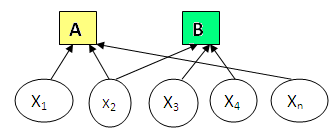
\includegraphics[scale=0.5]{bap.PNG}}
\caption{Bipartite Affiliation Graph}
\label{fig 1}
\end{figure}

A bipartite affiliation graph is denoted as $B(X,C,M)$,
with $X$ as the nodes, $C$ as the attribute value and $M$ denotes
the directed edge from $X$ to $C$ if node $X$ has attribute
value $C$. The problem now is to create a set of communities
$S = S_1, S_2, ..., S_k$ given $B(X,C,M)$. A parameter $p_c$ is
assigned to an attribute value $c \in C$. This is for calculating
the probability that a node $x_i$ has the attribute value $c$. This
can also be called the probability that a node $x_i$ belongs to
the same community as another $x_j$ having the value of a
particular attribute as $c$. The $P_A(i, j)$ denotes that the nodes
$i, j$ belong to the same community $A$. This can be shown by
the below equation.

\begin{equation}
P_A(i,j) = 1 - \prod_{c \in M_i \cap M_j} (1 - p_c)
\end{equation} 

Where,

\begin{itemize}
\item $M_i$ = node $i$ has membership to attribute value $c$.
\item $M_j$ = node $j$ has membership to attribute value $c$.\\
\end{itemize}

In Eqn. 1, the value of $P_A(i, j)$ is set to $\varepsilon$, following
the BIGCLAM procedure the value of $\varepsilon$ can be set as
$2|E|/|V|(|V| - 1)$ [21].


\subsection{Calculate the latent weights of the attributes}

Every attribute has its own importance or strength in
determining the cluster to which the node should belong to,
this is denoted here formally as $F_{uC}$. This is the strength
that attribute $C$ has for node $u$ in determining its cluster.
Considering this membership strength the Eqn. 1 can be
modified as follows:

\begin{equation}
P_A(i,j) = 1 - exp(-F_{uC}.F_{vC}^T)
\end{equation}

$F_{uC}$ is the membership strength of a single attribute,
similarly it is assumed that every node $i$ has a attribute
membership vector $F_i$ which contains the membership
strengths to all attributes in the data. The modified probability
that nodes $i, j$ now share a cluster is Eqn 2.\\


The intuition behind the above formula is simple, Consider
a node having attribute values same as the attribute values
of another node, in such a case the likelihood of both
nodes belonging to a particular community increases. This
means that for each attribute a pair of nodes shares we
get an independent chance of grouping the nodes. Thus,
naturally, the more attributes a pair of nodes shares, the
higher the probability of sharing the same community and
being connected.\\


 
If $M_u \cap M_v = 0$ then $P(u,v) = ε$ this is done to consider
cases where nodes might not share attributes but still are
connected. $F_u$ is the vector that denotes the strengths of
association of a node $u$ with each community in the network.
The task is to find the matrix of memberships $F$ that
maximizes the likelihood of generating the graph $G(V,E)$.
The log-likelihood of this is Eqn. 5. The Gradient update
algorithm is used to find the value of $F$ as shown in Eqn. 6 \\

\begin{equation}
l(F) = \sum_{u,v \in E} log(1 - \exp(-F_u.F_v^T)) - \sum_{u,v \notin E}(F_u.F_v^T)
\end{equation}
\begin{equation}
\bigtriangledown l(F_u) = \sum_{v \in N(u)} F_v \frac{\exp(-F_u.F_v^T)}{1 - \exp(-F_u.F_v^T)} - \sum_{v \notin N(u)} F_v
\end{equation}

\textbf{Decide Community Affiliation:} The membership strengths
matrix $F$ is computed from above and the next step is to
determine a suitable threshold above which it is possible to
determine whether the node i belongs to a community. This
threshold is $\delta$ set at
$\sqrt{−log(1 - \varepsilon)}$ [21]. The initialization
isn’t done using locally minimal neighborhoods approach of
BIGCLAM [21] as entity annotated attributes are used to get
initial values of the membership strengths $F_i$. The value of
$F_{i,k}$ is 0 if attribute $k$ is present and 0 if absent.\\

$\textbf{Choosing the number of communities:}$ This is done by
procedure specified in [23] where the model is trained using
an initial value of K. Then we detect K communities on the
80\% of node pairs and then evaluate the likelihood on the hold
out set. The K with the best hold out likelihood is used.

\subsection{Experimental Results}

\subsubsection{Artificial Neural Networks}
Artificial neural networks are composed of input layers, hidden layers and output layers. The number of hidden layers ideally should be more as they can compute more nonlinear relationships between the inputs. However, it is important to avoid over-fitting while deciding the number of hidden layers and the number of hidden units. The input feature matrix X and the weight matrix of the $W_{21}$ $(\theta_{1})$ and the result are given to the sigmoid function to decide which neurons of the hidden layer 1 i.e. ($a_{1}$) are activated. The output of this hidden layer is the multiplied with the second weight matrix $W_{31}$ $(\theta_{2})$ and so on till the output layer. The back-propagation algorithm is then used to obtain the adjusted weights. The cost function of the network for the classification problem is provided in Eqn. (1) and the penalty term (regularization) is used to it for preventing over-fitting is provided in Eqn.(2).\\



\subsubsection{Cost Function - Artificial Neural Networks}

The cost function is that of the standard regularized logistic regression which is generalized for k outputs instead of one output. For our problem the output is a single value of 0/1 depending upon whose influence in a network is more. The cost function shall be minimized using the backpropagation algorithm to get the ideal value of the weights.

\begin{equation}
J(\Theta ) = \frac{a}{b} \sum_{i=1}^{k}\sum_{k=1}^{k} * [-y_{k}^{i}*log((h_{\Theta }(x^{i}))_{k}) - (1-y_{k}^{(i)})*log((h_{\Theta }(x^{i}))_{k})] 
\end{equation}
\begin{equation}
Penalty =  \frac{\lambda }{m}* [\sum_{j=1}^{J1}\sum_{k=1}^{K1}*(\Theta _{(j,k))}^{(1))})^{2} + \sum_{j=1}^{J2}\sum_{k=1}^{K2}*(\Theta _{(j,k))}^{(2))})^{2}]
\end{equation}

\subsubsection{Gradient boosted trees}

Gradient boosting combines several weak learners into a strong learner using multiple iterations. Gradient boosting is applied with decision trees of fixed size as the first level learners. The decision tree partitions the input space into disjoint regions and predicts a constant value in each region. The General idea for a gradient boosted tree is to fit a model to the data i.e $F_1$(x) = y . Fit the model to the residuals denoted by $h_(1)$(x) = y - $F_1$(x). Then obtain a new model $F_2$(x) = $F_1$(x) + $h_1$(x). The value of 'm' or the hyper parameter which gives the number of iterations of the residual correction procedure is obtained by cross validation. \\ 





\subsubsection{Gradient Boosted trees}



Model Update rule:

\begin{equation}
F_{m}(x) = F_{(m-1)}(x)) + \sum_{j=1}^{J_m} \gamma_{jm} I (x \epsilon R_{jm}) 
\end{equation}

\subsection{Influence Ranking Algorithm}

The algorithm for comparison of influence between two users whose network features have been collected from Twitter is presented. The parameters of various models are set initially and these values are modified till the ideal values are obtained. The cross validation set is used for this purpose.\\

\begin{algorithm}
\caption{Influencer Ranking model}
\begin{algorithmic}[1]
 \State Set initial seed for random numbers
 \State Set the training control values
 \State Set the tuning grid for parameter search
 \For {each parameter set} do
 \For {each resampling iteration set} do
 \State hold out specific samples
 \State Pre process the data (Center and Scale)
 \State Fit the model on the remaining samples
 \State Predict the held out samples
 
 \EndFor
 \State Calculate the average performance across held out predictions
 \EndFor
 \State Determine the optimal parameter set
 \State Fit the final model to all the training data using optimal parameter set 
 

\end{algorithmic}
\end{algorithm}

\section{Experimental Study}

\subsection{Experiment setting}

The performance of the Influence Ranking algorithm in Section III-(C) is studied to understand the best set of features to measure influence.\\

\subsubsection{Dataset}  
The dataset, provided by Peer-index, comprises a standard, pair-wise preference learning task. Each data point describes two individuals whose identities are anonymized and their future references in the paper are made using labels 'A' and 'B'. For each person, 8 pre-computed, non-negative numeric features based on twitter activity are provided. The binary label represents a human judgement about which one of the two individuals is more influential. The Ground truth labels provided are 0/1 to indicate which of the users is more influential. The test set has 5952 entries for which label has to be predicted.

\begin{table}[!h]
\renewcommand{\arraystretch}{1.3}
\caption{Description of the dataset}
\label{table}
\centering
\begin{tabular}{|c|c|c|c|}
  \hline
\multicolumn{1}{|c|}{\textbf{Training set size}} & \multicolumn{1}{c|}{\textbf{Test set size}} & \multicolumn{1}{c|}{\textbf{Feature vector}} & \multicolumn{1}{c|}{\textbf{Classification}}\\
  \hline
  5500 & 5952 &  22 & Binary\\
  \hline
\end{tabular}
\end{table}


\subsection{Results}

The accuracy and performance on test set was measured for the Three layered ANN trained using correlated and uncorrelated predictors.

\begin{table}[H]
\renewcommand{\arraystretch}{1.3}
\caption{Modeling influence using Multilayered Perceptron with Backpropagation}
\label{table}
\centering
\begin{tabular}{|c|c|c|c|}
%\begin{tabular}{|p{0.1in}|p{0.75in}|p{0.51in}|p{.51in}|p{0.51in}|}
  \hline
\multicolumn{1}{|c|}{\textbf{Sample size}} & \multicolumn{1}{c|}{\textbf{Hidden units}} & \multicolumn{1}{c|}{\textbf{Training Accuracy}} & \multicolumn{1}{c|}{\textbf{Training Kappa}}\\
  \hline
  3521 &  16 & 72.29 & 44.55\\
  \hline
  3521 &  24 & 71.29 & 43.42\\
  \hline
  3521 &  32 & 71.55 & 43.04\\
  \hline
\end{tabular}
\end{table}

For above experiment correlated features ($\geq{0.75}$) were removed. Cross validation technique used was X-cross fold with X = 5 and 5 times repeat. Training set accuracy was used as selection criteria for evaluation and hidden units were decided as 16. The trained model gave an accuracy of 0.801 on the test set.


\begin{table}[!h]
\renewcommand{\arraystretch}{1.3}
\caption{Modeling influence using Multilayered Perceptron with Backpropagation}
\label{table}
\centering
\begin{tabular}{|c|c|c|c|}
  \hline
\multicolumn{1}{|c|}{\textbf{Sample size}} & \multicolumn{1}{c|}{\textbf{Hidden units}} & \multicolumn{1}{c|}{\textbf{Training Accuracy}} & \multicolumn{1}{c|}{\textbf{Training Kappa}}\\
  \hline
  3521 &  22 & 73.11 & 46.19\\
  \hline
  3521 &  33 & 72.96 & 45.89\\
  \hline
  3521 &  44 & 73.08 & 46.14\\
  \hline
\end{tabular}
\end{table}


For above experiment correlated features were allowed for training. Cross validation technique used was X-cross fold with X = 5 and 5 times repeat. Training set accuracy was used as selection criteria for evaluation and hidden units were decided as 22. The trained model with 22 hidden nodes gave accuracy of 0.81 on test set.


Modeling influence using Decision trees with gradient boosting was performed. To tune the parameters of the trees such as Number of Trees $N_{trees}$, Shrinkage, Interaction depth and Minimum observations in nodes, a grid search was conducted. Training set Accuracy was the criteria to select the optimal model. Fig. 2 shows the performance of the algorithm during grid search and the accuracy is seen in Fig. 2 to degrade as the interaction depth increases beyond 5 and the shrinkage is increased beyond 0.1.  The final parameter values for the optimal model obtained through grid search were $N_{trees}$ = 110, interaction depth = 5, shrinkage = 0.1 and minimum observations in nodes = 20. The accuracy obtained on the test set was 0.8601.\\

Random forests (Rf) technique to model influence using the correlated features and removing correlation was performed. Advantage of random forests models are better accuracy but at the cost of interpret-ability of the model. The tuning parameter is Number of trees for these model whose value has to be determined empirically. The final model selected using training set accuracy had classification accuracy of 0.856 on the test set. The model with correlated features gave slightly better result 0.859. Removing correlation doesn’t improve accuracy on this dataset for the ANN and Rf.\\

Improving accuracy using ensembling, boosting or bagging at the cost of interpret-ability is a disadvantage for implementation. Such techniques have improved accuracy but such models obtained had more theoretical importance than practical value as seen in the NetFlix competition. Table V contains the training set and test set accuracy of greedy ensembles of GBM Trees, Random forests and ANN obtained in Section IV-B. The test set accuracy of the models is used as the selection criteria and Extreme Gradient Boosting has the highest accuracy on the test set at 0.87. ROC curves to denote the performance of Ensembled models of ANN, GBM, Rf is shown in Fig 3 and Area under curve is used as the selection criteria to obtain the optimal model. The results are shown for each combination in Fig. 3. The correlation between the predictions of GBM and Rf is 0.88 and so their ensemble was discarded due to highly correlated predictions. The highest accuracy on the test set is seen for the ensemble of GBM and Rf as shown in Table V.  \\

\begin{table}[!h]
\renewcommand{\arraystretch}{2.5}
\caption{Ensembled Predictors}
\label{table}
\centering
\begin{tabular}{|p{0.1in}|p{0.75in}|p{0.51in}|p{.51in}|}
  \hline
\multicolumn{1}{|c|}{\textbf{Sr. No}} & \multicolumn{1}{c|}{\textbf{Technique}} & \multicolumn{1}{c|}{\textbf{Training Accuracy}} & \multicolumn{1}{c|}{\textbf{Test set Accuracy}}\\
  \hline
  1 & Boosting &  0.7856 & 0.82 \\
  \hline
  2 & Greedy Ensemble (ANN,GBM,RF) &  0.86 & 0.867 \\
  \hline
  3 & Greedy Ensemble (GBM,RF) &  0.86 & 0.83 \\
    \hline
  4 & Averaging Predictors (GBM,RF) &  0.79 & 0.866 \\
    \hline
  5 & Extreme Gradient Boosting &  0.79 & 0.87 \\
  \hline
\end{tabular}
\end{table}








\section{Conclusion}
The framework for ranking influential nodes in a social network based on characteristics obtained from a nodes interaction on the social network has been presented in this paper. The influence is modeled using machine learning techniques unlike the conventional influence maximization approaches. Features of the individual nodes obtained from its interaction characteristics  are used and the network architecture is not considered. The performance metrics of the algorithms used in the experiments is classification accuracy and using this objective criteria Extreme Gradient Boosted decision tree has shown the highest accuracy. The influence ranking algorithm in this paper is a suitable technique for computation of the influence score of various nodes and this has been validated by the extensive experiments performed on Twitter dataset.   







% trigger a \newpage just before the given reference
% number - used to balance the columns on the last page
% adjust value as needed - may need to be readjusted if
% the document is modified later
%\IEEEtriggeratref{8}
% The "triggered" command can be changed if desired:
%\IEEEtriggercmd{\enlargethispage{-5in}}

% references section

% can use a bibliography generated by BibTeX as a .bbl file
% BibTeX documentation can be easily obtained at:
% http://mirror.ctan.org/biblio/bibtex/contrib/doc/
% The IEEEtran BibTeX style support page is at:
% http://www.michaelshell.org/tex/ieeetran/bibtex/
%\bibliographystyle{IEEEtran}
% argument is your BibTeX string definitions and bibliography database(s)
%\bibliography{IEEEabrv,../bib/paper}
%
% <OR> manually copy in the resultant .bbl file
% set second argument of \begin to the number of references
% (used to reserve space for the reference number labels box)
\begin{thebibliography}{}

\bibitem{fah}
Fahad, A., Alshatri, N., Tari, Z., Alamri, A., Khalil, I., Zomaya, A.Y., Foufou, S. and Bouras, A., 2014. A survey of clustering algorithms for big data: Taxonomy and empirical analysis. IEEE transactions on emerging topics in computing, 2(3), pp.267-279.

 \bibitem{jain}
Jain, A.K., 2010. Data clustering: 50 years beyond K-means. Pattern recognition letters, 31(8), pp.651-666.

\bibitem{bez} 
Bezdek, J.C., Ehrlich, R. and Full, W., 1984. FCM: The fuzzy c-means clustering algorithm. Computers and Geosciences, 10(2-3), pp.191-203.

\bibitem{frah} 
Fraley, C. and Raftery, A.E., 2002. Model-based clustering, discriminant analysis, and density estimation. Journal of the American statistical Association, 97(458), pp.611-631.

\bibitem{est} 
Ester, M., Kriegel, H.P., Sander, J. and Xu, X., 1996, August. A density-based algorithm for discovering clusters in large spatial databases with noise. In KDD (Vol. 96, No. 34, pp. 226-231).

\bibitem{ank} 
Ankerst, M., Breunig, M.M., Kriegel, H.P. and Sander, J., 1999, June. OPTICS: ordering points to identify the clustering structure. In ACM Sigmod record (Vol. 28, No. 2, pp. 49-60). ACM.

\bibitem{ros}
Rosvall, Martin, and Carl T. Bergstrom. "Maps of random walks on complex networks reveal community structure." Proceedings of the National Academy of Sciences 105.4 (2008): 1118-1123.
\bibitem{pon}
Pons, Pascal, and Matthieu Latapy. "Computing communities in large networks using random walks." International Symposium on Computer and Information Sciences. Springer Berlin Heidelberg, 2005.
\bibitem{clau}
Clauset, Aaron, Mark EJ Newman, and Cristopher Moore. "Finding community structure in very large networks." Physical review E 70, no. 6 (2004): 066111.
\bibitem{newn}
M. E. J. Newman, Fast algorithm for detecting community structure in networks. Phys. Rev. E 69, 066133 (2004).
\bibitem{mnew}
Newman, Mark EJ, and Michelle Girvan. "Finding and evaluating community structure in networks." Physical review E 69.2 (2004): 026113.
\bibitem{ragh}
Raghavan, Usha Nandini, Réka Albert, and Soundar Kumara. "Near linear time algorithm to detect community structures in large-scale networks." Physical review E 76.3 (2007): 036106.
\bibitem{blon}
Blondel, and Vincent D., et al. "Fast unfolding of communities in large networks." Journal of statistical mechanics: theory and experiment 2008.10 (2008): P10008.
\bibitem{reic}
Reichardt, Jörg, and Stefan Bornholdt. "Statistical mechanics of community detection." Physical Review E 74.1 (2006): 016110.
\bibitem{mark}
Newman, Mark EJ. "Finding community structure in networks using the eigenvectors of matrices." Physical review E 74.3 (2006): 036104.


\bibitem{liu} Liu, Y., Niculescu-Mizil, A., and Gryc, W. (2009, June). Topic-link
LDA: joint models of topic and author community. In proceedings of the
26th annual international conference on machine learning (pp. 665-672).
ACM.

\bibitem{bal} Balasubramanyan, R., \& Cohen, W. W. (2011, April). Block-LDA:
Jointly modeling entity-annotated text and entity-entity links. In Proceed-
ings of the 2011 SIAM International Conference on Data Mining (pp.
450-461). Society for Industrial and Applied Mathematics.

\bibitem{xu} Xu, W., Liu, X., \& Gong, Y. Document clustering based on non-negative
matrix factorization. In Proceedings of the 26th annual international ACM
SIGIR conference on Research and development in information retrieval
(pp. 267-273). ACM.

\bibitem{for} Fortunato, S. and Hric, D., 2016. Community detection in networks: A
user guide. Physics Reports, 659, pp.1-44.
\bibitem{fani} Fani, Hossein, and Ebrahim Bagheri. ”Community detection in social
networks.” Encyclopedia with Semantic Computing and Robotic Intelli-
gence 1.01 (2017): 1630001.
\bibitem{one} Yang, J. and Leskovec, J., 2013, February. Overlapping community
detection at scale: a nonnegative matrix factorization approach. In Pro-
ceedings of the sixth ACM international conference on Web search and
data mining (pp. 587-596). ACM.
\bibitem{two} Yang, J., McAuley, J. and Leskovec, J., 2013, December. Community
detection in networks with node attributes. In Data Mining (ICDM), 2013
IEEE 13th international conference on (pp. 1151-1156). IEEE.
\bibitem{three} Yang, J., McAuley, J. and Leskovec, J., 2014, February. Detecting
cohesive and 2-mode communities indirected and undirected networks. In
Proceedings of the 7th ACM international conference on Web search and
data mining (pp. 323-332). ACM.
\bibitem{gry} Grygorash, O., Zhou, Y., \& Jorgensen, Z. (2006, November). Minimum
spanning tree based clustering algorithms. In Tools with Artificial Intelli-
gence, 2006. ICTAI’06. 18th IEEE International Conference on (pp. 73-
81). IEEE.



\end{thebibliography}




% that's all folks
\end{document}


